%\newpage
\section{Omówienie wyników testów}

Zaprojektowane algorytmy sterowania przetestowano na 3 przykładowych scenariuszach ruchu uszeregowanych pod kątem stopnia trudności.

\subsection{Scenariusz 1 - Wykrywanie kolizji}

W pierwszym scenariuszu zbadano zdolność pojazdów do unikania kolizji. Do wykrywania kolizji pojazdy wykorzystywały czujniki laserowe. Po wykryciu zbliżającej się kolizji, pojazd zatrzymywał się. Po zniknięciu kolizji (np. gdy poprzedzający pojazd ruszył) samochód ruszał ponownie. Przykładowe migawki z symulacji przedstawiono poniżej.

\begin{figure}[!h]
	\centering
	\centering
	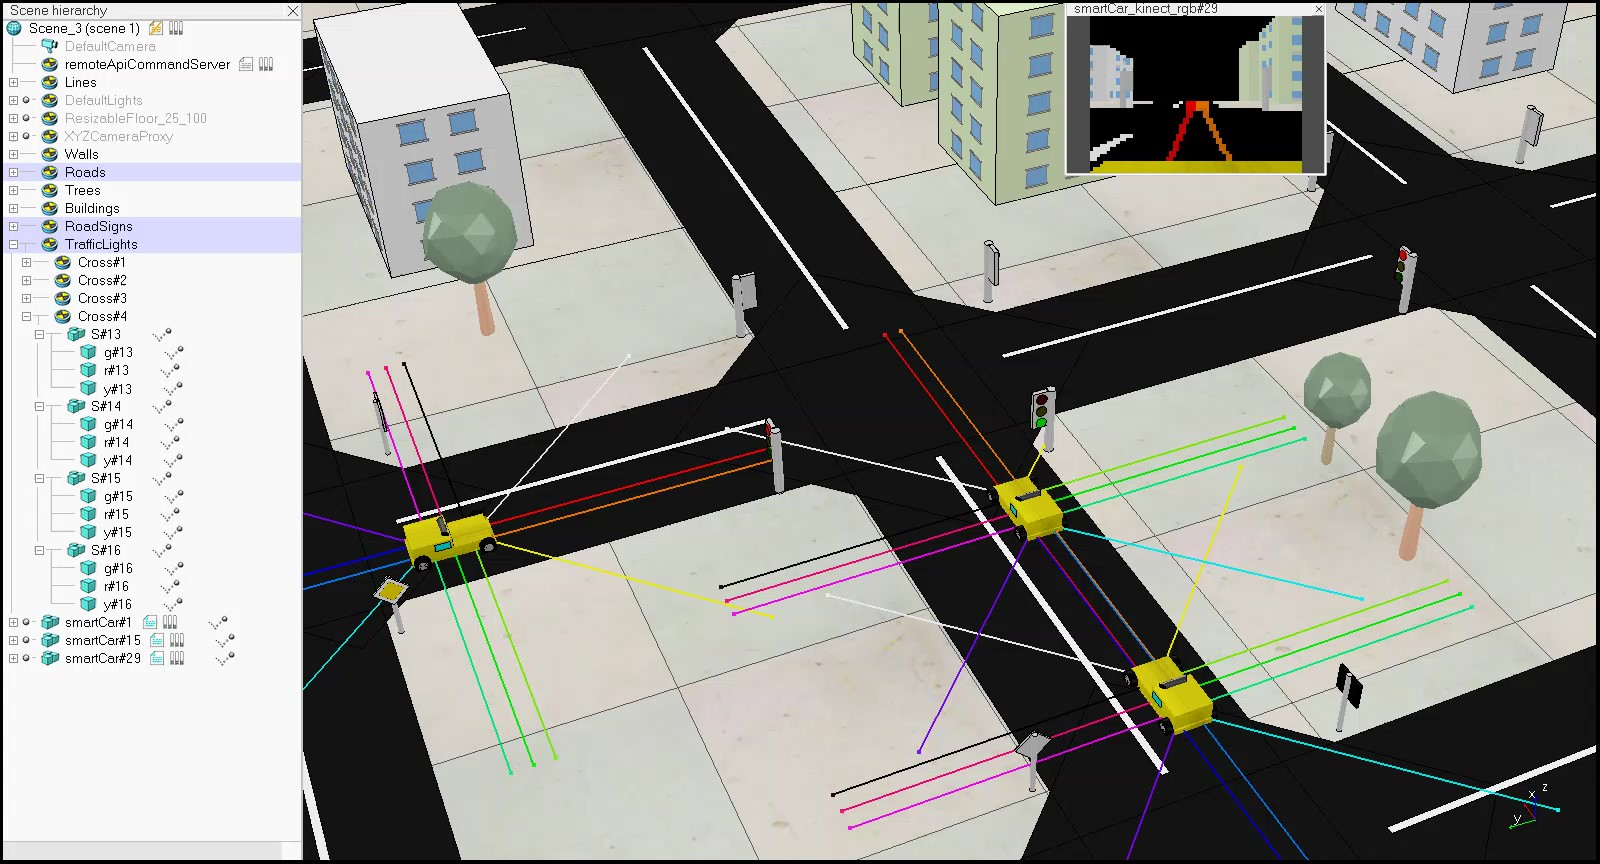
\includegraphics[width=.8\linewidth]{p11.jpg}
	\caption{Początek symulacji - scen. 1}
	\label{fig:p11}
\end{figure}

\begin{figure}[!h]
	\centering
	\centering
	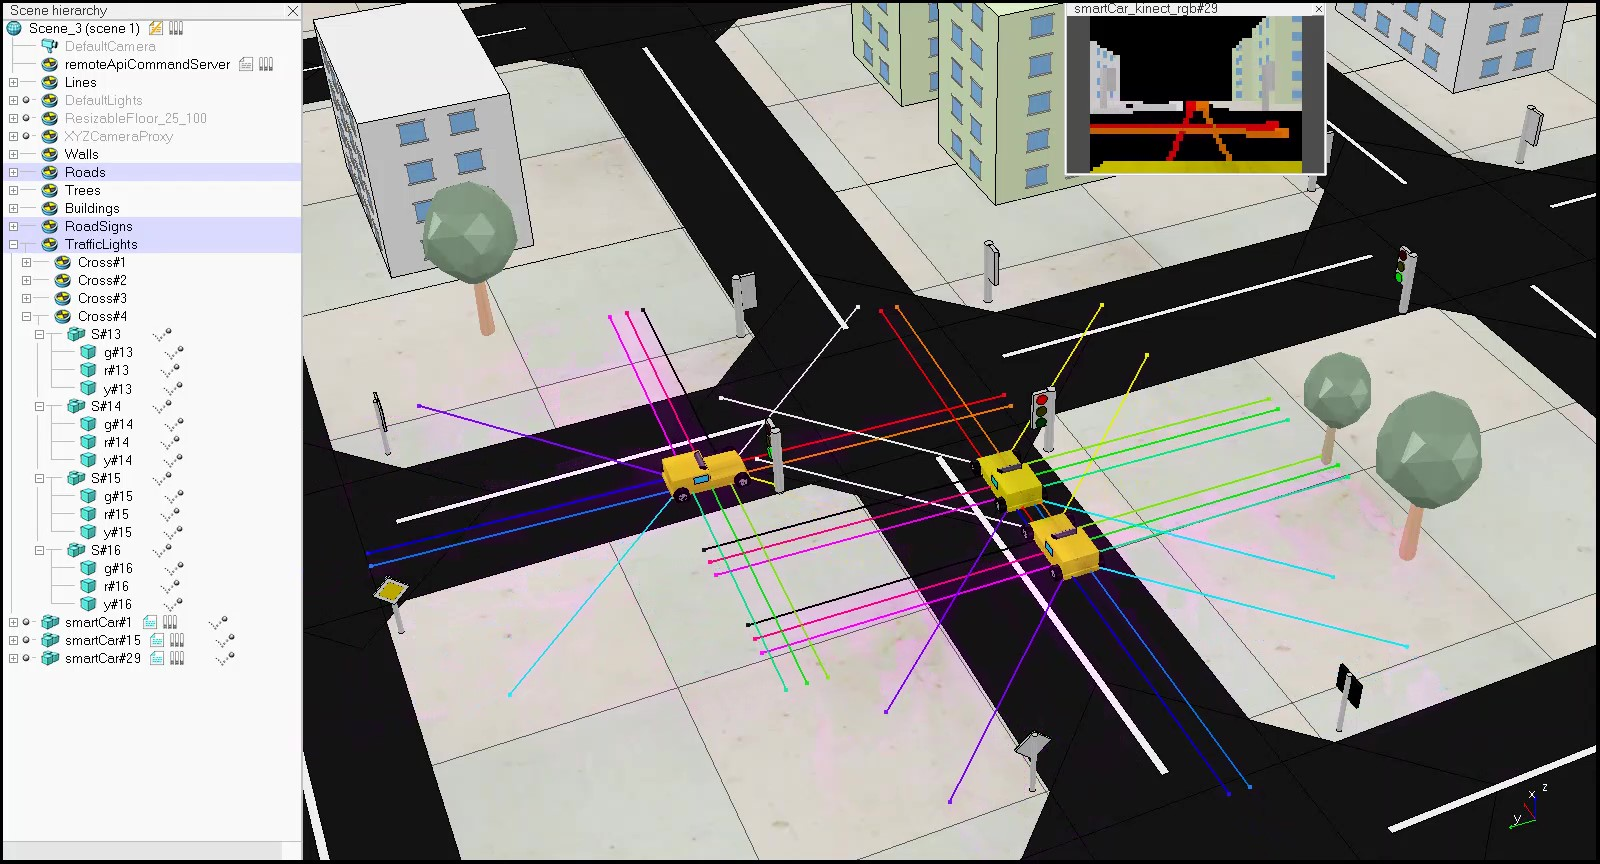
\includegraphics[width=.8\linewidth]{p12.jpg}
	\caption{Wykrycie kolizji po dojeździe do skrzyżowania - scen. 1}
	\label{fig:p12}
\end{figure}

\subsection{Scenariusz 2 - Pokonywanie skrzyżowań}

W drugim scenariuszu zbadano zdolność pojazdów do pokonywania skrzyżowań. Samochody pokonywały skrzyżowania zgodnie z pierwszeństwem wyznaczanym przez zawczasu ustalony priorytet dróg. Samochody zatrzymywały się przed skrzyżowaniem w momencie gdy na drodze o wyższym priorytecie znajdowały się samochody zbliżające się do skrzyżowania. Przykładowe migawki z symulacji przedstawiono poniżej.

\begin{figure}[!h]
	\centering
	\centering
	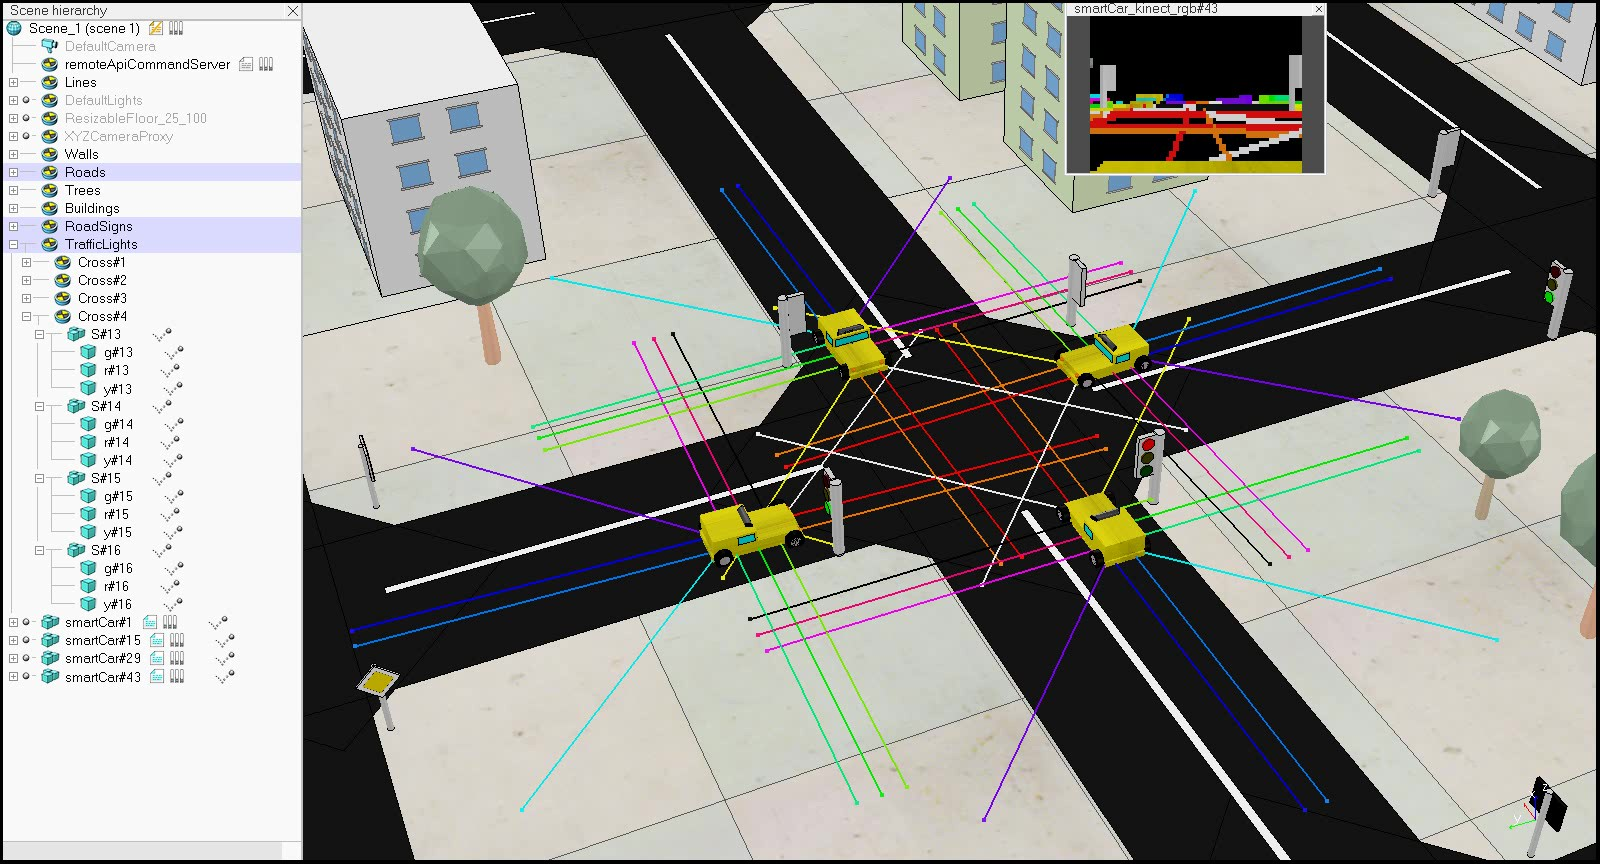
\includegraphics[width=.8\linewidth]{p21.jpg}
	\caption{Początek symulacji - scen. 2}
	\label{fig:p21}
\end{figure}

\begin{figure}[!h]
	\centering
	\centering
	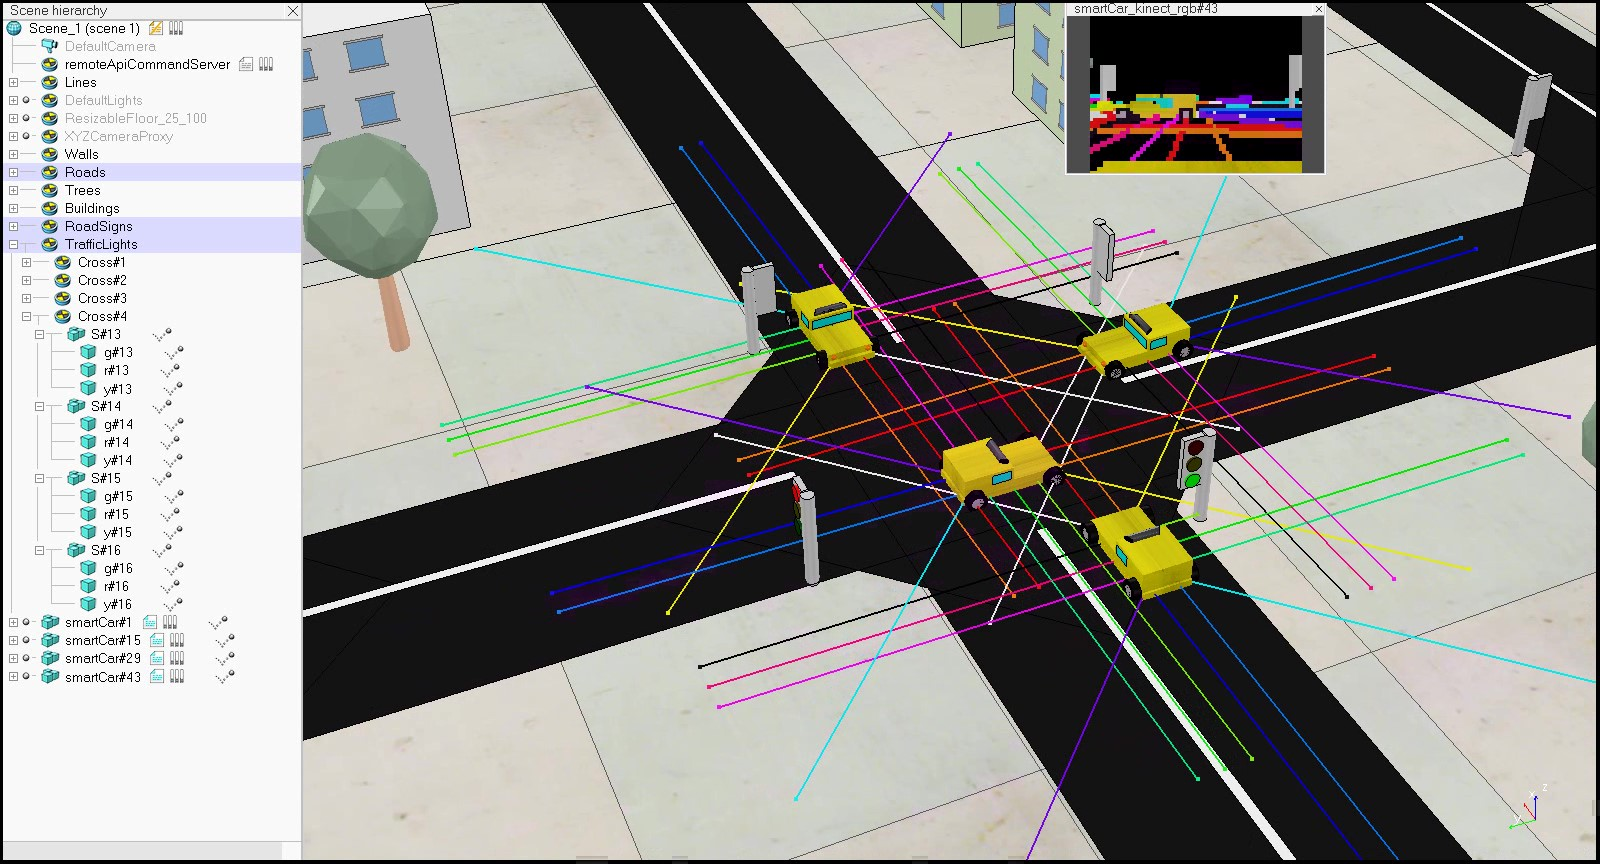
\includegraphics[width=.8\linewidth]{p22.jpg}
	\caption{Przejazd 1. samochodu przez skrzyżowanie - scen. 2}
	\label{fig:p22}
\end{figure}

\begin{figure}[!h]
	\centering
	\centering
	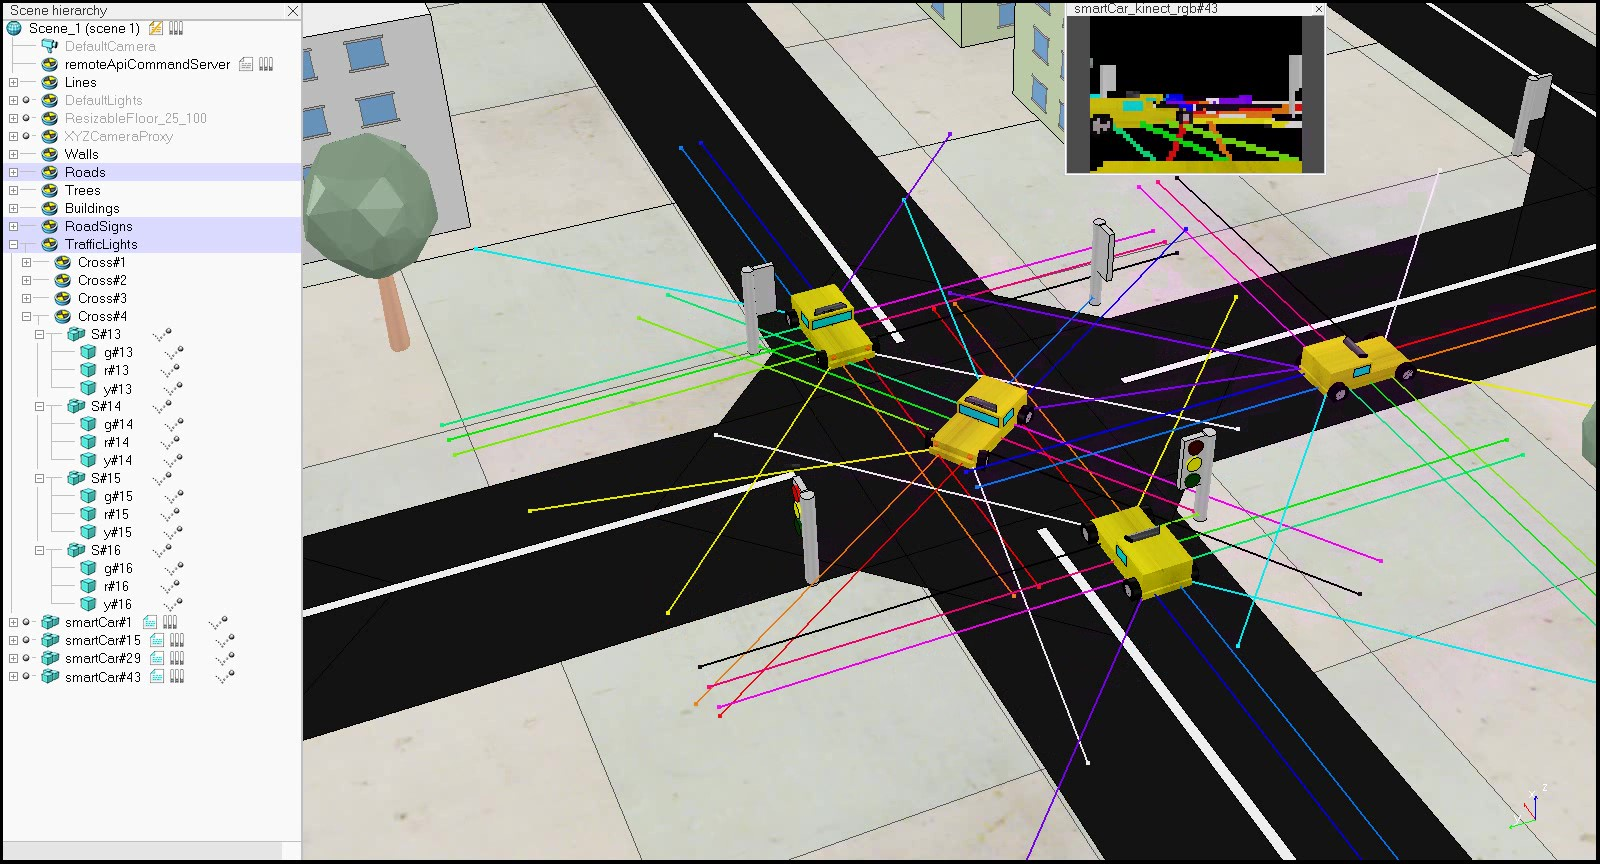
\includegraphics[width=.8\linewidth]{p23.jpg}
	\caption{Skręt w lewo 2. samochodu przez skrzyżowanie - scen. 2}
	\label{fig:p23}
\end{figure}

\begin{figure}[!h]
	\centering
	\centering
	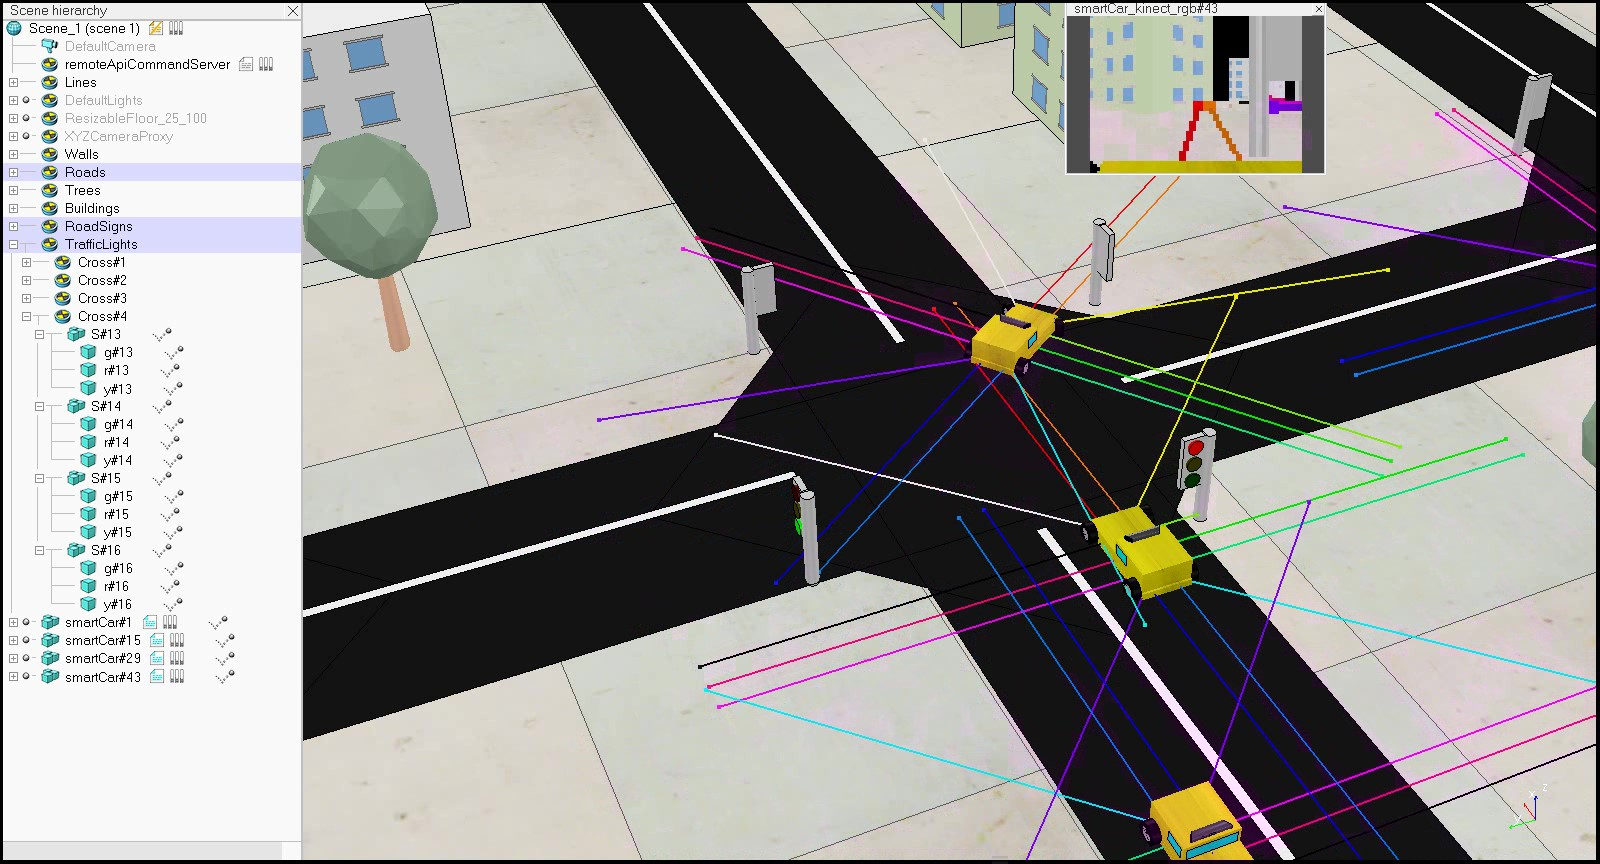
\includegraphics[width=.8\linewidth]{p24.jpg}
	\caption{Zawracanie 3. samochodu na skrzyżowaniu - scen. 2}
	\label{fig:p24}
\end{figure}

\begin{figure}[!h]
	\centering
	\centering
	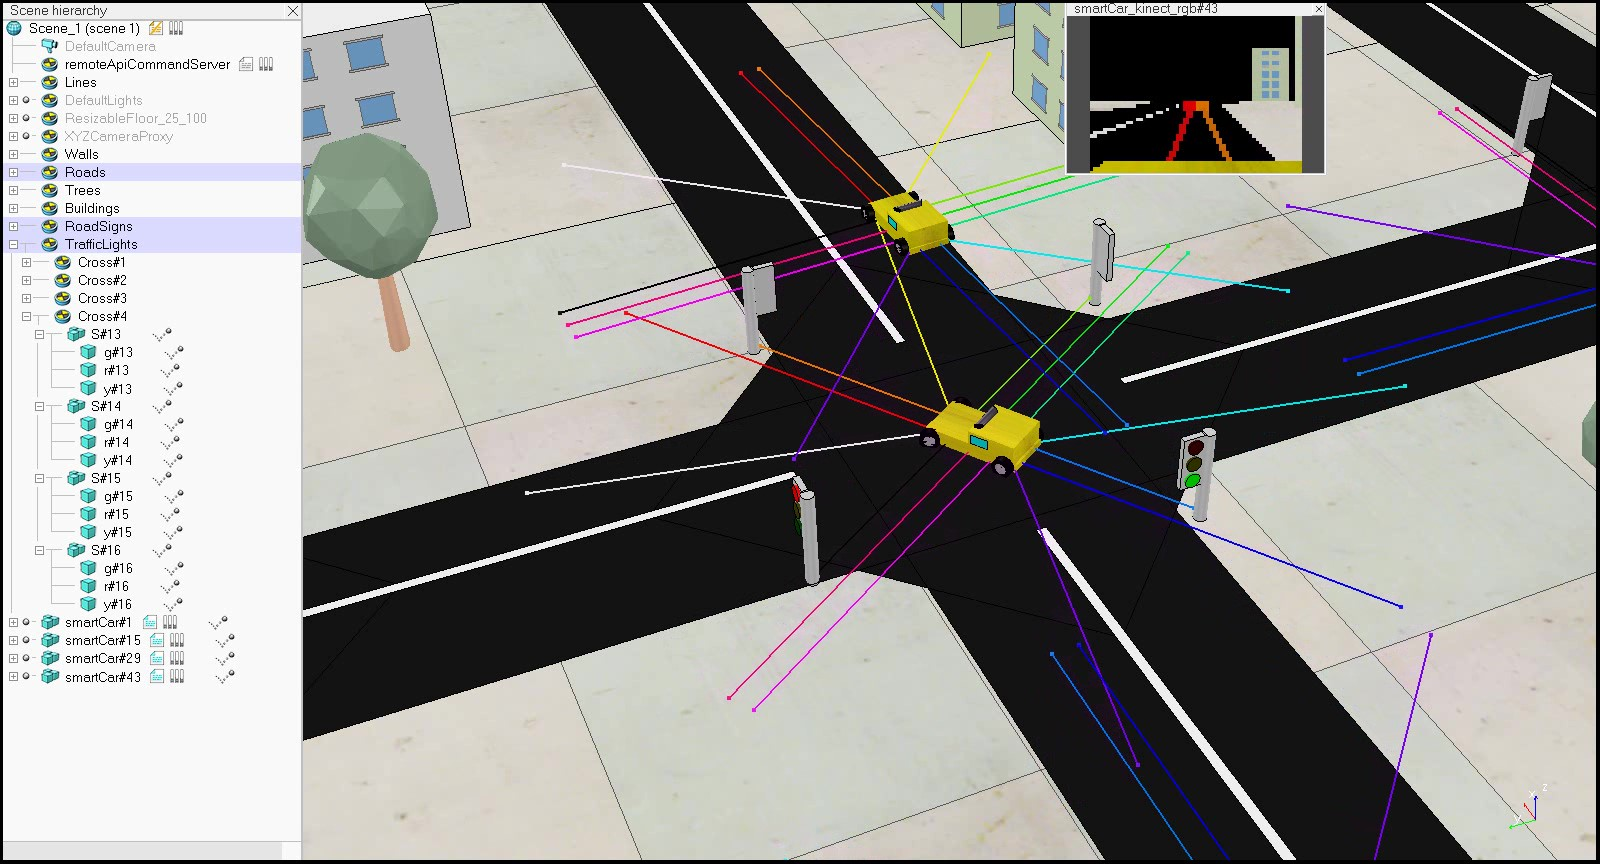
\includegraphics[width=.8\linewidth]{p25.jpg}
	\caption{Zawracanie 4. samochodu na skrzyżowaniu - scen. 2}
	\label{fig:p25}
\end{figure}

\subsection{Scenariusz 3 - Przejazd pojazdów do punktów docelowych}
 
 W ostatnim scenariuszu zbadano zdolność pojazdów do pokonywania zadanych tras w obliczu dużego ruchu. Przeprowadzono symulację z 8 samochodami, którym punkty docelowe zadano w sposób losowy. Przykładowe migawki z symulacji przedstawiono poniżej.
 
 \begin{figure}[!h]
 	\centering
 	\centering
 	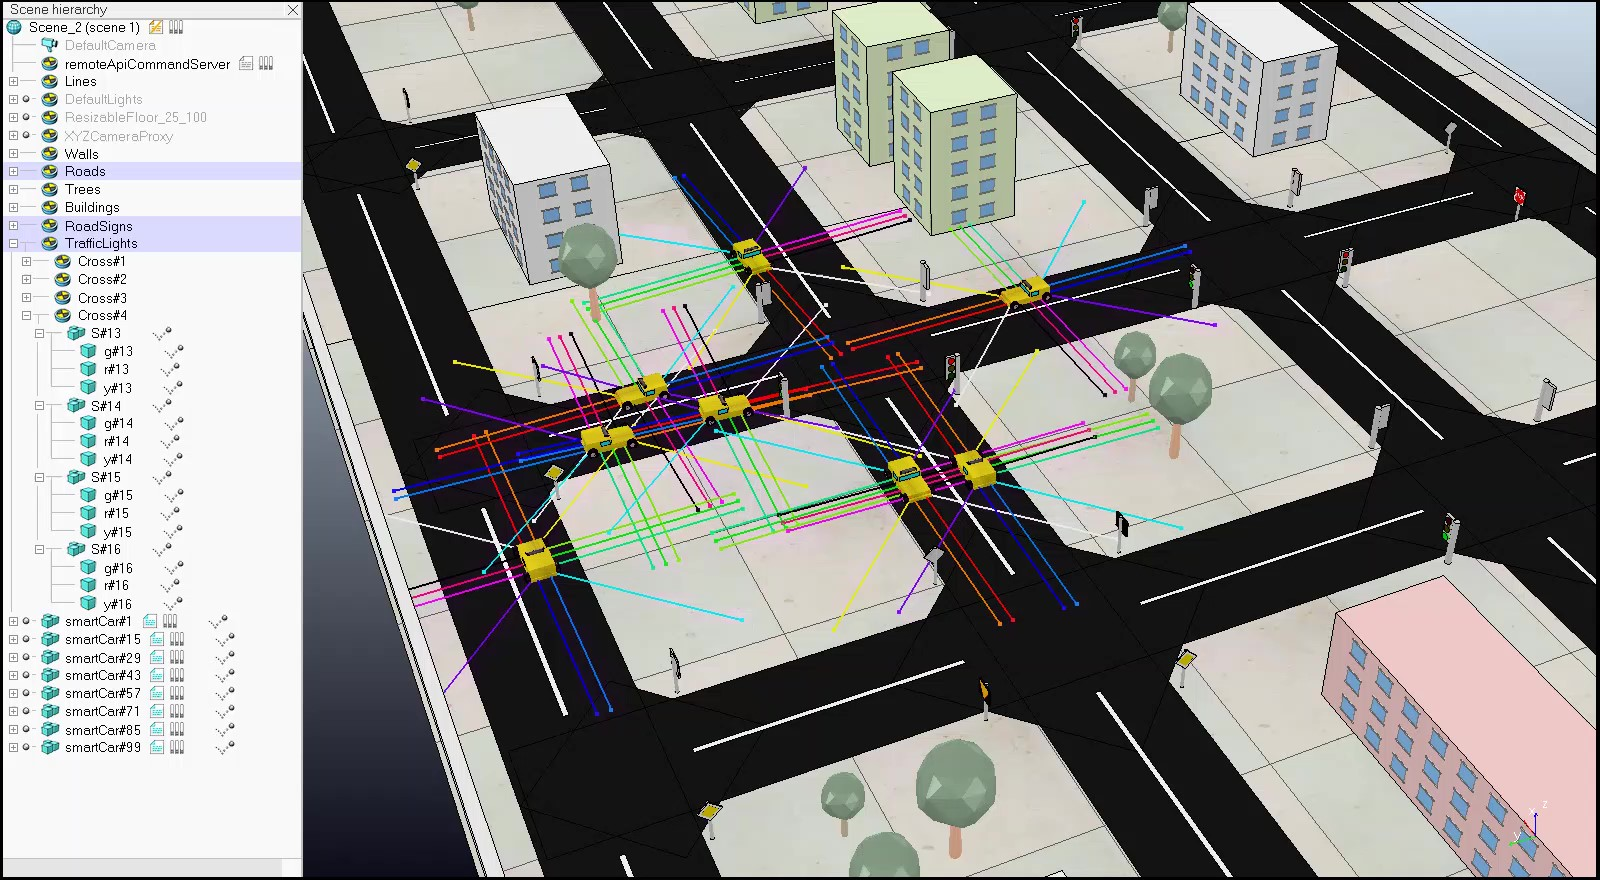
\includegraphics[width=.8\linewidth]{p31.jpg}
 	\caption{Początek symulacji - scen. 3}
 	\label{fig:p31}
 \end{figure}

 \begin{figure}[!h]
	\centering
	\centering
	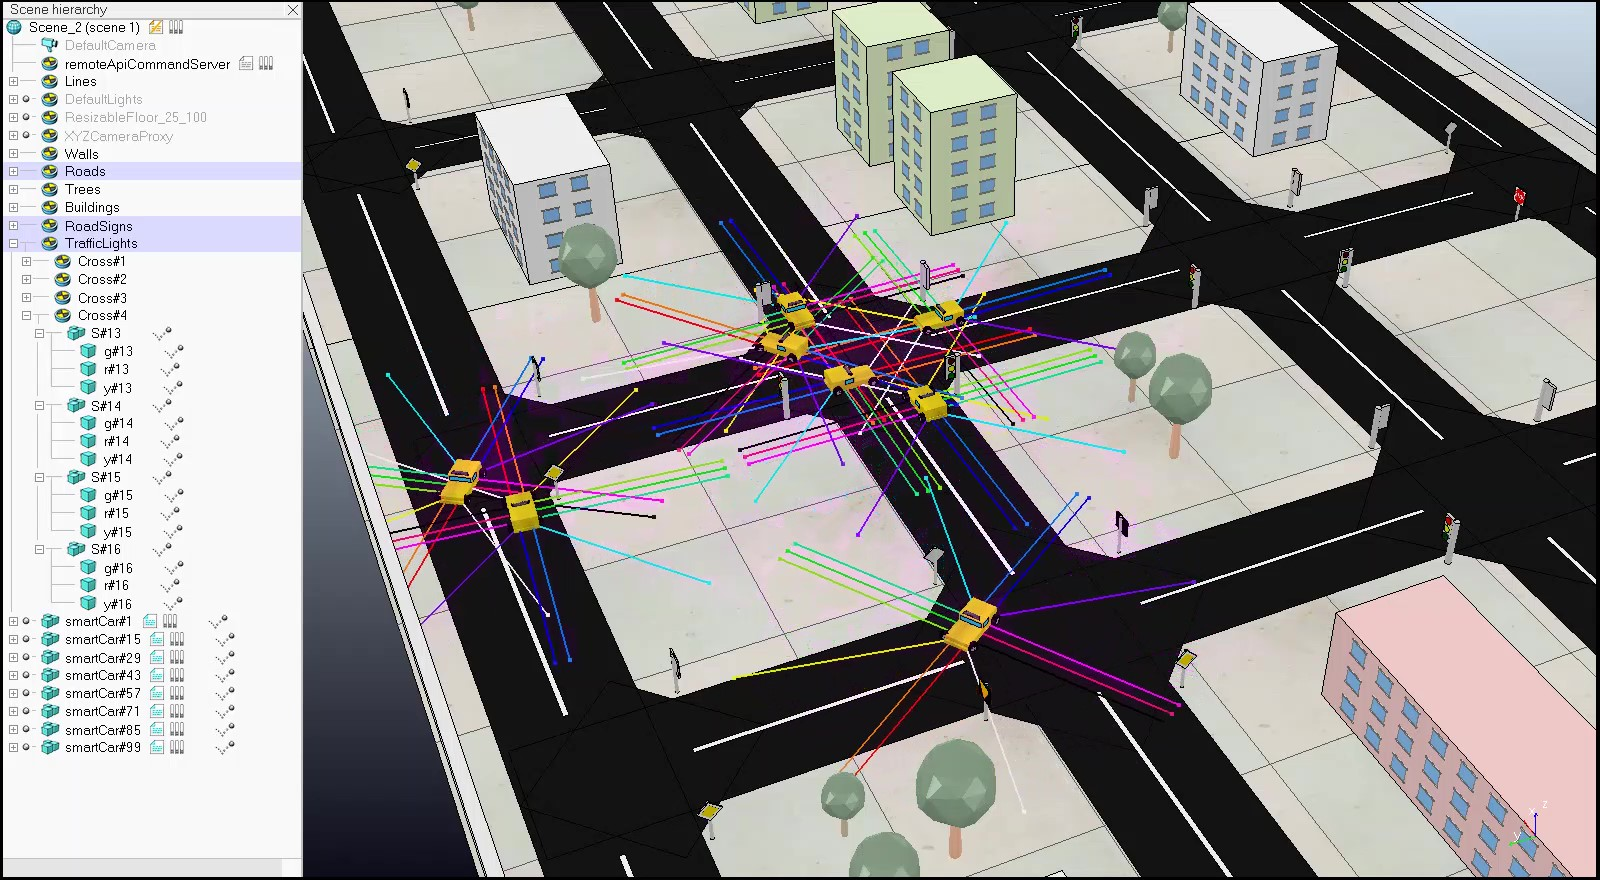
\includegraphics[width=.8\linewidth]{p32.jpg}
	\caption{Migawka z symulacji - scen. 3}
	\label{fig:p32}
\end{figure}

 \begin{figure}[!h]
	\centering
	\centering
	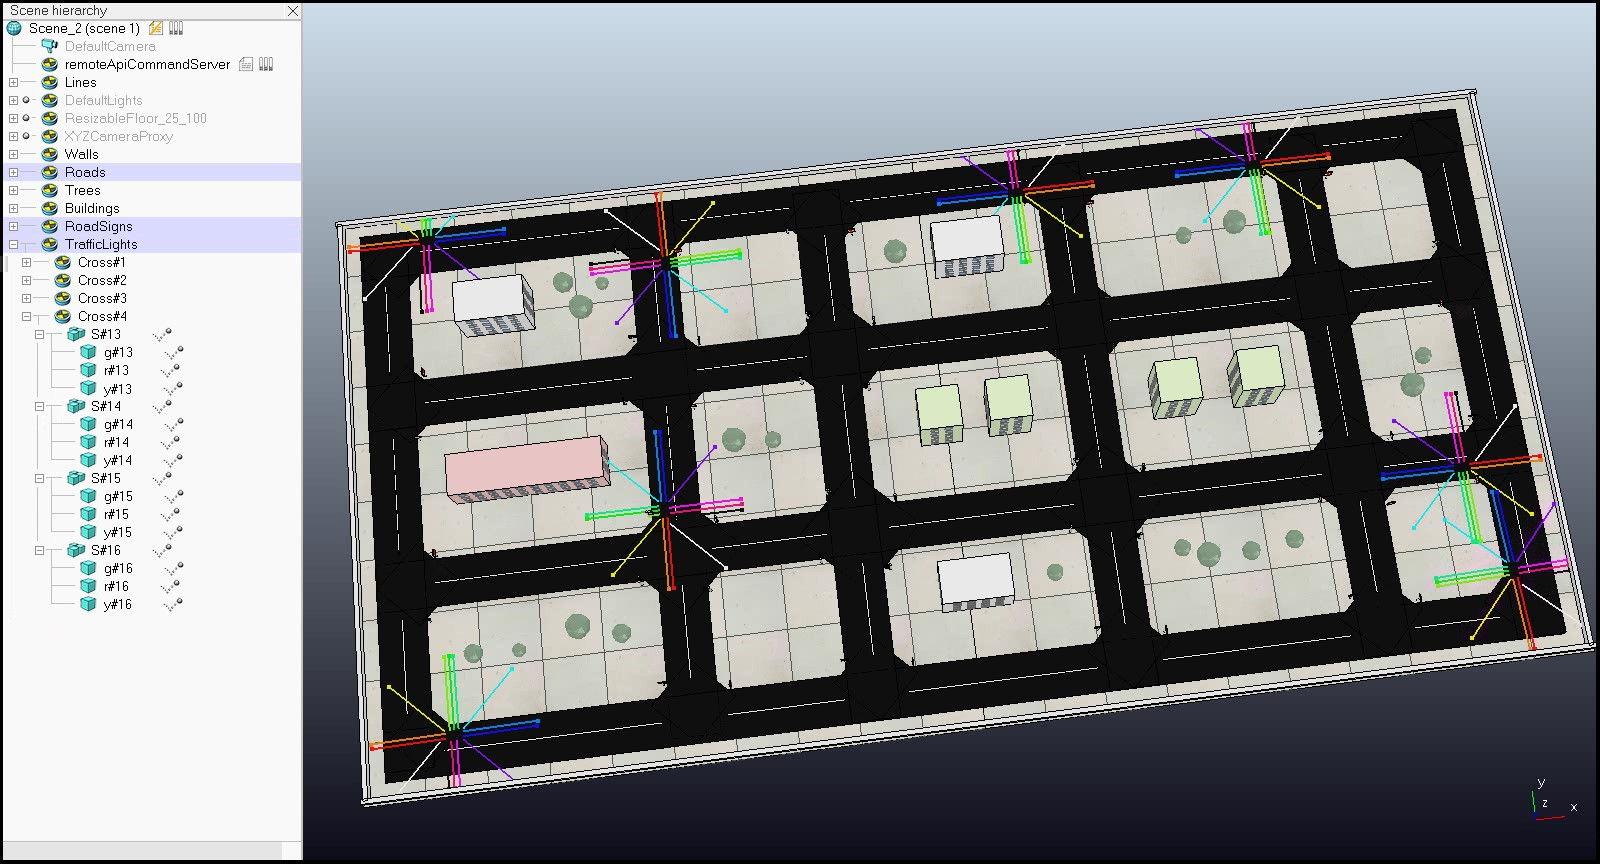
\includegraphics[width=.8\linewidth]{p33.jpg}
	\caption{Koniec symulacji - zaznaczone końcowe pozycje - scen. 3}
	\label{fig:p33}
\end{figure}
 
 
 
